\chapter{Zweiter Ansatz: Ethereum} % Main chapter title

\label{eth} % For referencing the chapter elsewhere, use \ref{eth} 

\section{Grundlagen}
Ethereum ist genau wie Bitcoin ein Peer-to-Peer Netzwerk Protokoll, dass auf einer öffentlichen Blockchain basiert und einen Systemzustand verwaltet. Es handelt sich im Gegensatz zu Bitcoin um eine generalisierte Blockchain die nicht nur Finanztransaktionen speichern kann, sondern sogenannte Smart Contracts\footnote{Bitcoin Transaktionen beinhalten im Grunde auch Smart Contracts allerdings sind diese weniger Mächtig. Abschnitt \ref{eth_grundlagen_btc_diff} geht genauer auf die Unterschiede zwischen Bitcoin und Ethereum ein.}. Ethereum sieht sich als eine Open Source Plattform, die es ermöglicht dezentrale Applikationen zu entwickeln und bereitzustellen.

\subsection{Smart Contracts}
Ethereum ermöglicht es Geschäftsprozesse in Form von Smart Contracts zu programmieren und von einem globalen dezentralen Netzwerk ausführen zu lassen. Ein Contract ist ein Programm bestehend aus einer Reihe von Anweisungen, die ausgeführt werden, sobald das Programm eine Nachricht in Form einer Transaktion erhält. Contracts haben die Möglichkeit Daten aus der Blockchain auszulesen und auf ihr Daten zu speichern. Smart Contracts können sowohl von Menschen als auch von anderen Contracts ausgelöst werden. Contracts können daher mit anderen Contracts über die vom Programmierer festgelegte Schnittstelle interagieren. Es handelt sich bei einem Smart Contract also nicht um einen Vertrag, der erfüllt werden muss, sondern um ein öffentliches Stück Software, dass den Zustand eines Ethereum Accounts verwaltet.
\subsection{Ethereum Accounts}
Um Ethereum nutzen zu können braucht man einen Account. Ethereum Accounts bestehen aus:\\
\begin{itemize}
\item Einer 20 Byte langen Adresse,
\item einem Kontostand in Ether(siehe Abschnitt \ref{eth_ether}),
\item einem Nonce-Wert der sicherstellt, dass Transaktionen nur einmal ausgeführt werden können,
\item Smart Contract Code (optional),
\item und Speicherplatz (optional).
\end{itemize} In Ethereum gibt es zwei Arten von Accounts. Die erste Art ist eine Adresse, die, wie bei Bitcoin, durch den Besitz des privaten Schlüssels kontrolliert wird. Diese Art von Account wird durch eine Wallet Software verwaltet. Die zweite Art ist ein  Contract Account, der durch den Smart Contract Code kontrolliert wird. Der Smart Contract Code verwaltet eigenständig den Kontostand des Accounts und verhält sich genau so, wie der Programmierer es festgelegt hat.

\subsection{Transaktionen}
Interaktionen mit dem Ethereum Netzwerk finden in Form sogenannter Transaktionen statt. Transaktionen sind, durch den privaten Schlüssel eines Ethereum Account, signierte Datenpakete, die eine Nachricht(siehe Abschnitt \ref{eth_messages}) beinhalten. Transaktionen beinhalten:
\begin{itemize}
\item den Empfänger der Nachricht,
\item eine digitale Signatur, die den Absender der Nachricht identifiziert,
\item eine Anzahl an Ether, die an den Empfänger versandt wird,
\item Daten (Bytes), die vom Contract ausgelesen werden können (optional),
\item einen sogenannten Gas-Wert, der die maximale Anzahl Rechenschritte festlegt, die die Transaktion bei der Ausführung nutzen darf
\item und den GAS-Preis, der festlegt, wie viel der Absender bereit ist für die Ausführung eines Rechenschritts der Transaktion zu zahlen.
\end{itemize}

Es gibt zwei verschiedene Arten von Transaktion. Sie unterscheiden sich durch die in der Transaktion angegebene Empfangsadresse. 
Wird die Empfangsadresse durch einen privaten Schlüssel kontrolliert, handelt es sich lediglich um eine Finanztransaktion, die Ether vom Sender zum Empfänger Account transferiert. Anderenfalls handelt es sich um eine Transaktion, die den Contract Code der Empfangsadresse ausführt. Welche Funktion ausgeführt werden soll, wird vom Sender im Datenfeld der Transaktion kodiert.

\subsection{Nachrichten}\label{eth_messages}
Bei Nachrichten handelt es sich um virtuelle Objekte, die im Gegensatz zu Transaktionen nicht abgespeichert werden, sondern lediglich in der Ethereum Virtual Machine (siehe Abschnitt \ref{eth_evm}) verwendet werden. \if lediglich zur Interaktion mit dem Contract Code eines Smart Contracts verwendet werden.\fi Ein weiterer Unterschied ist, dass Transaktionen im Gegensatz zu Nachrichten immer von ''außen'' erzeugt werden. Nachrichten können hingegen auch von Smart Contracts erzeugt werden. Nachrichten bestehen aus einem impliziten Sender, einem Empfänger, einem Ether-Betrag, einem Gas-Wert und einem optionalen Datenfeld. Genau wie bei Transaktionen führt das versenden von Nachrichten zu der Ausführung des Conrtact Codes der Empfangsadresse.

\subsection{Ether}\label{eth_ether} 
Ether ist die Kryptowährung des Ethereum Netzwerks. Sie entsteht wie bei Bitcoin durch Mining und wird benutzt, um für Transaktionsgebühren und die Ausführung von Contract Code zu bezahlen. Ether bildet durch die Zuhilfenahme des Gas-Werts und Gas-Preis den anti Spam Schutz des Ethereum Netzwerks.
\subsubsection{Gas-Wert}
Da Smart Contracts Schleifen beinhalten und andere Smart Contracts durch Nachrichten aufrufen können, muss sichergestellt werden, dass die Ausführung terminiert. Da es für den Sender der Transaktion schwierig, in manchen Fällen sogar unmöglich\footnote{Beispielsweise wenn der nächste Block eine Transaktion enthält, die bewirkt, dass die eigentlichen Transaktion ein unterschiedlicher Code-Pfad durchlaufen wird.} ist, die Anzahlt Schritte der Ausführung im Vorhinein zu wissen, legt der Absender durch den Gas-Wert die maximale Anzahl Rechenschritte fest, die die Transaktion bei der Ausführung dauern darf.
\subsubsection{Gas-Preis}
Durch den Gas-Preis gibt der Sender einer Transaktion an, wie viel Ether er pro Rechenschritt bereit ist zu bezahlen. Die Ausführung einer Transaktion kann einen Ethereum Account somit um maximal \code{Gas-Wert * Gas-Preis} Ether belasten.

\subsection{Ethereum Virtual Machine}\label{eth_evm} 
In der Ethereum Virtual Machine wird der Smart Contract Code ausgeführt. Sie arbeitet die Anweisungen des Contracts der Reihe nach ab und bricht ab, falls der Gas-Wert nicht für die Ausführung der Transaktion ausreicht. Durch das sequenzielle Abarbeiten der Transaktionen eines Blocks wird der Systemzustand nach und nach von der Ethereum Virtual Machine angepasst.
\begin{figure}[H]
\centering
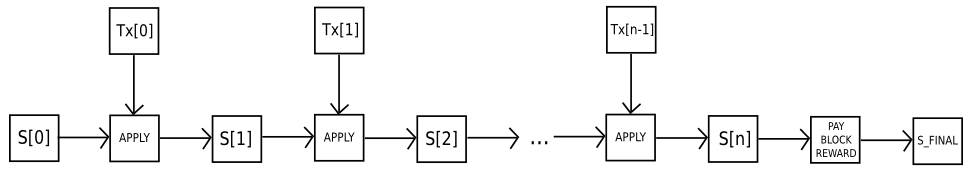
\includegraphics[width=1\linewidth]{Figures/eth/ETH_txn_statetransformation}
\decoRule
\caption{Veränderung des Systemzustand}
\label{fig:ETH_txn_statetransformation}
\end{figure}
Der Systemzustand wird bei Ethereum durch den Zustand aller Ethereum Accounts beschrieben. 

\subsection{Systemzustand Übergangsfunktion}
Die Ethereum Virtual Machine geht bei der Abarbeitung einer Transaktion folgendermaßen vor:
\begin{enumerate}
\item Sie prüft ob die Transaktion gemäß der Konsensregeln korrekt formatiert ist, eine valide Signatur besitzt und ob der Nonce-Wert der Transaktion mit dem Nonce-Wert des Absender-Accounts übereinstimmt. Ist eine dieser Vorbedingungen nicht erfüllt, wird die Bearbeitung der Transaktion abgebrochen. 
\item Es wird die maximal fällige Transaktionsgebühr durch das Multiplizieren des Gas-Werts mit dem Gas-Preis berechnet. Anschließend wird geprüft, ob der Account des Senders genug Ether besitzt, um die berechnete Transaktionsgebühr zu bezahlen. Ist dies der Fall wird die maximale Transaktionsgebühr vom Sender-Account abgezogen. Anderenfalls wird die Bearbeitung der Transaktion abgebrochen. 
\item Nun wird der Gas-Wert der Transaktion um einen gewissen Betrag jedes Transaktionsbyte verringert. Der Sender zahlt auf diese Weise für den Platz, den die Transaktion in der Blockchain einnimmt.
\item Der Ether Wert der Transaktion wird vom Sender auf den Empfänger Account überwiesen. Falls der Empfänger Account noch nicht existiert wird er angelegt. Wird der Empfänger Account durch einen Smart Contract verwaltet, wird der Contract Code entweder vollständig ausgeführt oder aufgrund fehlenden Gas abgebrochen. 
\item Falls der Sender nicht genug Ether oder verbleibendes Gas für die Überweisung besitzt, werden alle bisherigen Veränderungen des Systemzustands rückgängig gemacht. In diesem Fall wird ausschließlich die Transaktionsgebühr  auf den Account des Miners überschrieben.
\item Im erfolgreichen Fall werden die Gebühren des verbleibenden Gas an den Sender zurückerstattet und die Gebühren des verbrauchten Gas an den Account des Miners überschrieben.
\end{enumerate}

\subsection{Systemzustand Beispiel}
Das folgende Beispiel betrachtet, wie das Anwenden eine Transaktion einen alten Systemzustand in einen neuen Systemzustand überführt. 
\begin{figure}[H]
\centering
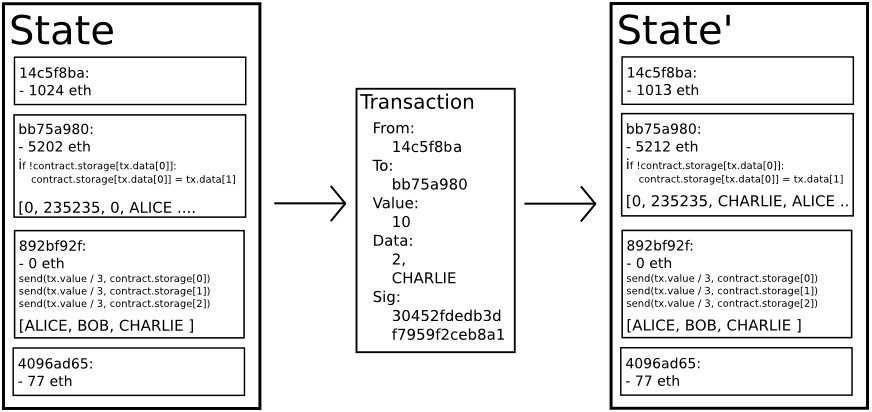
\includegraphics[width=1\linewidth]{Figures/eth/ETH_statetransition_example}
\decoRule
\caption{Veränderung des Systemzustand}
\label{fig:ETH_statetransition_example}
\end{figure}
Die in Abbildung \ref{fig:ETH_statetransition_example} betrachtete Transaktion ruft den Smart Contract des Accounts der Adresse \code{bb75a980} auf. Angenommen die Transaktion überweist einen Betrag von 10 Ether, besitzt einen Gas-Wert von 2000, einen Gas-Preis von 0,001 Ether, enthält 64 Bytes an Daten(\code{data[0]=2,data[1]='CHARLIE'}) und besitzt eine Gesamtgröße von 170 Bytes. Dann erfolgt die Abarbeitung der Transaktion folgendermaßen:
\begin{enumerate}
\item Es wird durch die Prüfung der Signatur einerseits sichergestellt, dass die Daten der Transaktion nicht manipuliert wurden und andererseits, dass die Überweisung der 10 Ether vom Besitzer des Accounts \code{14c5f88a} autorisiert wurde. 
\item Da der Account des Senders über \code{2000 * 0,001 = 2} Ether besitzt, wird die Bearbeitung der Transaktion fortgesetzt und die 2 Ether vom Account des Senders abgezogen.
\item Unter der Annahme, dass man 5 Gas pro Transaktionsbyte bezahlen muss, wird der Gas-Wert von 2000 auf 1150 Gas verringert. (170 Bytes * 5 = 850 Gas) 
\item Der Transaktionsbetrag von 10 Ether wird vom Sender Account \code{14c5f88a} auf den Account \code{bb75a980} überwiesen.
\item Nun wird der Conract Code des Empfängeraccounts ausgeführt:\\ \code{if !contract.storage[tx.data[0]]: contract.storage[tx.data[0]] = tx.data[1]}\\
Da der Speicherplatz des Contracts an Stelle 2 noch nicht verwendet ist, wird  der Wert \code{CARLIE} aus den Transaktionsdaten abgespeichert. Unter der Annahme, dass diese Operationen 150 Gas verbrauchen ergibt sich ein verbleibender Gas-Wert von \code{1150 -150 = 1000}. 
\item Die verbleibenden \code{1000 * 0,001 = 1} Ether werden auf den Account des Senders zurücküberwiesen und die Anpassung des Systemzustands ist fertig\footnote{Im resultierenden Systemzustand aus Abbildung \ref{fig:ETH_statetransition_example} fehlt die an den Miner gezahlte Transaktionsgebühr von 1 Ether. Diese zahlt sich der Miner wie in Abbildung \ref{fig:ETH_txn_statetransformation} gezeigt in der letzten Transaktion zusammen mit den restlichen Transaktionsgebühren des Blocks aus.}.
\end{enumerate}

\subsection{Unterschiede zu Bitcoin}\label{eth_grundlagen_btc_diff} 
\subsubsection{Turing-Vollständigkeit}
Bitcoin besitzt intern auch eine Skript-Sprache zur Ausführung von Transaktionen. Diese ist im Gegensatz zu Ethereum bewusst eingeschränkt und nicht turingmächtig. Da man keine Schleifen programmieren kann, führt dies dazu, dass man Code mehrfach wiederholen muss. Dies führt dazu, dass Transaktionen die Smart Contracts ausdrücken in Bitcoin mehr Platz in der Blockchain einnehmen. Ethereum muss sich aufgrund der Turing-Vollständigkeit um das Halteproblem kümmern. Durch die Angabe eines maximalen Gas-Werts stellt Ethereum sicher, dass die Ausführung einer Transaktion spätestens nach einer gewissen Zeit abgebrochen wird. 
\subsubsection{Betrags-Blindheit}
Der Betrag, der einer Bitcoin-Adresse zugeschrieben wird, kann entweder nur ganz oder gar nicht ausgegeben werden. Dies ist bei Ethereum nicht der Fall. Der Nonce-Wert des Ethereum Accounts verhindert, dass eine Transaktion nicht zweimal ausgeführt werden kann.
\subsubsection{Blockchain-Blindheit}
In Bitcoin kann man bei der Ausführung der Transaktionen nicht auf Blockchain Daten wie Beispielsweise vorherige Blockhash-Werte, Zeitstempel oder None-Werte zugreifen. Eine Transaktion, die einen vorherigen Blockhash ausließt und als Zufallsquelle verwendet ist mit der Bitcoin Skript-Sprache nicht möglich.
\subsubsection{Fehlender Zustand}
Die Ethereum Accounts ermöglichen es einen weitaus komplexeren Systemzustand abzubilden. Bei Bitcoin besteht der Systemzustand lediglich aus der Menge aller Adressen, die Bitcoins besitzen.